\section{Theorie}
\label{sec:theorie}

Das Element Rubidium zählt zur Gruppe der Alkalimetalle und ist für den Versuch des Optischen Pumpens deshalb besonders geeignet.
Denn ähnlich wie das Wasserstoffatom besitzen Alkalimetalle nur ein Valenzelektron.
Die anderen Elektronen sind in vollen Schalen und tragen nicht zu dem optischen Pumpen bei.\\
In diesem Versuch werden zwei Isotope des Rubidiums verwendet.
Das stabile Rubidium $^{85}\text{Rb}$ und der radioaktive Beta-Strahler $^{87}\text{Rb}$ liegen als Gas vor.

\subsection{Feinstruktur}
Die Quantenzahlen der beiden Isotope unterscheiden sich kaum, bis auf den Kernspin I.\\
Der Gesamtbahndrehimpuls J berechnet sich aus dem Drehimpuls L und dem Spin S nach $\vec{J} = \vec{L} + \vec{S}$.
Dabei sind die Quantenzahlen gegeben durch $|L-S|$ bis $|L+S|$ in ganzen Schritten.
Im Fall des Rubidium ergibt sich in jedem Fall $J=\sfrac{1}{2}$.
In \autoref{tab:quanten} sind alle Quantenzahlen im Grundzustand ohne Zeeman-Aufspaltung aufgelistet.

\begin{table}[H]
    \centering
    \begin{tabular}{c c c}
        \toprule
        - & $^{85}\text{Rb}$ & $^{87}\text{Rb}$\\
        \midrule
        L & 0 & 0\\
        S & $\sfrac{1}{2}$ & $\sfrac{1}{2}$\\
        J & $\sfrac{1}{2}$ & $\sfrac{1}{2}$\\
        I & $\sfrac{5}{2}$ & $\sfrac{3}{2}$\\
        F & 2;3 & 1;2\\
        \bottomrule
    \end{tabular}
    \caption{Diese Tabelle listet die Quantenzahlen der Rubidium Isotope dar, inklusive des Kernspins I und des Gesamtimpulses F, die zu der Hyperfeinstruktur gehören.}
    \label{tab:quanten}
\end{table}

Im ersten angeregten Zustand verändert sich der Bahndrehimpuls zu $\text{L}=1$, was als 2p Zustand bekannt ist.\\
Die Kurzschreibweise für den Zustand ist durch
\begin{equation}
    ^{2S+1}L_J
\end{equation}
gegeben, wobei L der Buchstabe des Zustandes ist.\\
Der Grundzustand wird also beschrieben als $^2S_{\sfrac{1}{2}}$ und der erste angeregte Zustand als $^2P_{\sfrac{1}{2}}$.
Die Feinstruktur ist in \autoref{fig:fein} graphisch dargestellt.

\begin{figure}[H]
    \centering
    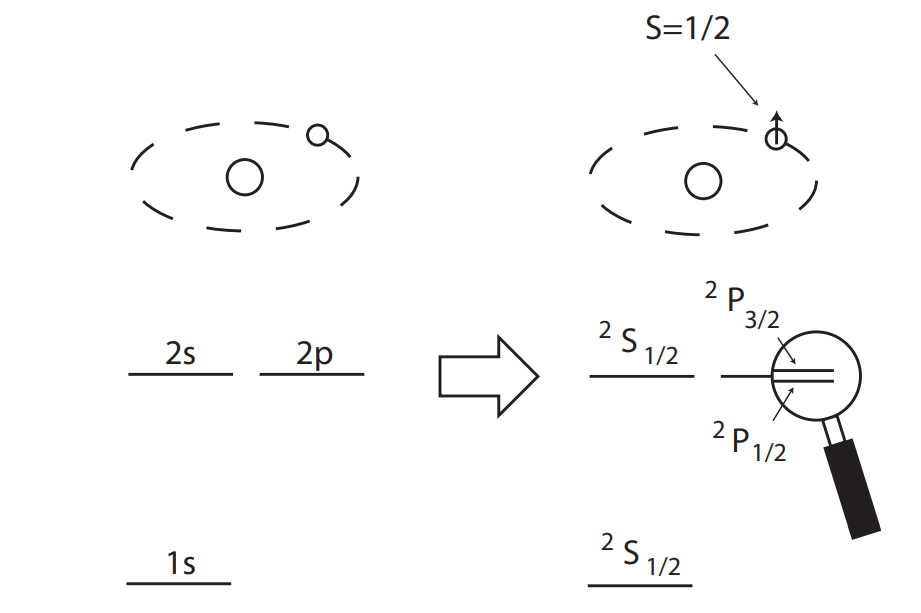
\includegraphics[scale=0.4]{figures/feinstruktur.png}
    \caption{In dieser Abbildung ist die Feinstruktur schematisch dargestellt.\cite{pdf_anleitung}}
    \label{fig:fein}
\end{figure}

\subsection{Hyperfeinstruktur}
Bei der Hyperfeinstruktur wird zusätzlich der Kernspin I betrachtet.
Zusammen mit dem Gesamtdrehimpuls berechnet sich der Gesamtimpuls des Rubidiums mit $\vec{F} = \vec{J} + \vec{I}$.\\
Hierbei ist die Kopplung dieselbe, die auch die Spin-Bahn hat, also berechnet sich die Quantenzahl mit $|I-J|$ bis $|I+J|$.
Es ergeben sich für die zwei Isotope verschiedene Gesamtimpulsquantenzahlen, wie in \autoref{tab:quanten} gelistet ist.
In \autoref{fig:hyper} wird die Hyperfeinaufspaltung von $^{87}\text{Rb}$ dargestellt.\\
Der Grundzustand $^2S_{\sfrac{1}{2}}$ ist in der Abbildung nicht dargestellt, wird jedoch aufgrund des gleichen Gesamtbahndrehimpulses $\text{J}=\sfrac{1}{2}$, auch gleich aufgespalten wie $^2P_{\sfrac{1}{2}}$.

\begin{figure}[H]
    \centering
    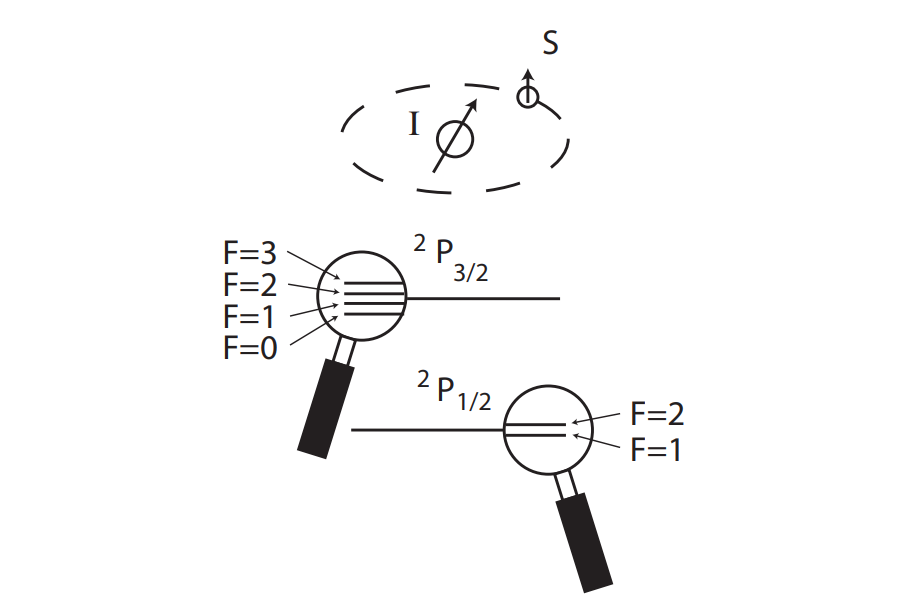
\includegraphics[scale=0.4]{figures/hyperfeinstruktur.png}
    \caption{In dieser Abbildung ist die Hyperfeinstruktur von $^{87}\text{Rb}$ schematisch dargestellt.\cite{pdf_anleitung}}
    \label{fig:hyper}
\end{figure}

\subsection{Zeeman-Aufspaltung}
Die Zeeman-Aufspaltung ist nach dem niederländischen Physiker Pieter Zeeman benannt, der für dessen Entdeckung 1902 den Nobelpreis erhielt.
Der Zeeman Effekt tritt auf, wenn ein äußeres Magnetfeld die Energieniveaus einzelner Zustände von Atomen verschiebt, und dadurch Aufspaltungen in den Spektrallinien bildet.\\
Das äußere Magnetfeld wechselwirkt mit der magnetischen Atomhülle, die sich aus der Kopplung von Spin der Elektronen und dem Bahndrehimpuls (L-S-Kopplung) zusammensetzt.
Einen wesentlich kleineren Beitrag leistet der Kernspin I.\\
Die Wechselwirkungsenergie ist gegeben durch:

\begin{equation}
    \Delta E_{\text{Z},F} = g_F \mu_B M B
    \label{eq:zeeman}
\end{equation}
mit dem Bohr'schen Magneton $\mu_B$ und dem Landé-Faktor
\begin{equation}
    g_F = g_J \cdot \frac{F(F+1) + J(F+1) - I(I+1)}{2F(F+1)}
    \quad \text{,} \quad
    g_J = \frac{3J(J+1) + S(S+1) - L(L+1)}{2J(J+1)}
    \label{eq:landefaktor}
\end{equation}

Die Quantenzahl $M$ beschreibt den aufgespaltenen Zustand, dessen Differenz zum Energieniveau der Hyperfeinaufspaltung das $\Delta E_{\text{Z},F}$ angibt.\\
In \autoref{fig:zeeman} ist die Aufspaltung graphisch dargestellt.

\begin{figure}[H]
    \centering
    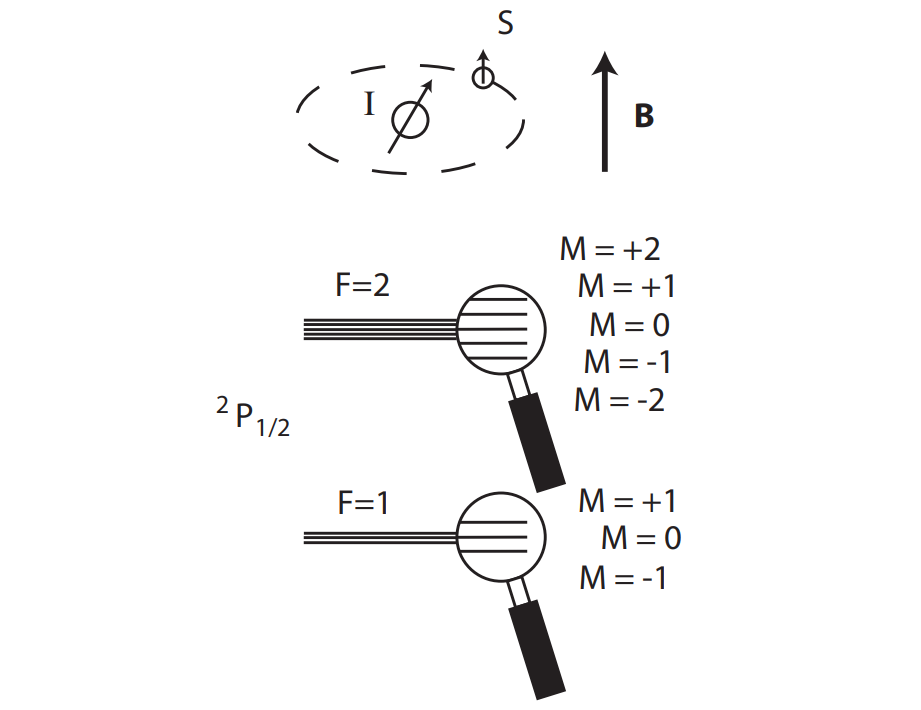
\includegraphics[scale=0.4]{figures/zeeman.png}
    \caption{In dieser Abbildung ist die Zeeman-Aufspaltung von $^{87}\text{Rb}$ graphisch dargestellt.\cite{pdf_anleitung}}
    \label{fig:zeeman}
\end{figure}

\subsubsection{Quadratischer Zeeman-Effekt}
Bei hohen externen Magnetfeldern können abgeschlossene Schalen in den Atomen nicht mehr vernachlässigt werden, da diese ebenfalls ein magnetisches Moment ausbilden.
Dadurch erweitert sich die Wechselwirkungsenergie,

\begin{equation}
    \Delta E_{\text{QZ},F} = g_F^2\ \mu_{\text{B}}^2\ \frac{1-2M}{\Delta E_{\text{hyp}}}\ B^2
    \label{eq:quadzeeman}
\end{equation}

wobei $\Delta E_{\text{hyp}}$ den Niveauunterschied in der Hyperfeinaufspaltung angibt.

\subsection{Optisches Pumpen}
Der Ausdruck \enquote{Optisches Pumpen} bezeichnet die elektromagnetische Stimulation von Atomen, dessen Valenzelektronen gleichverteilt auf den Zeeman-Niveaus liegen.
Diese Elektronen haben durch die Stimulation geregelte Zustände innerhalb der Niveaus, die sie annehmen können.
Solche Auswahlregeln betreffen die Absorption von Strahlung, sowie die Emission.
\subsubsection{Auswahlregeln}{
Es gilt für die Differenz von Endzustand und Anfangszustand $\Delta$:
\begin{itemize}
    \item $\Delta F = \pm 1$
    \item $\Delta M = +1 \quad$ , für zirkular rechts polarisiertes Licht
    \item $\Delta M = 0 \quad$ , für linear polarisiertes Licht
    \item $\Delta M = -1 \quad$ , für zirkular links polarisiertes Licht
\end{itemize}}
Angeregte Elektronen bleiben nicht für immer in ihren Niveaus, sondern relaxieren von selbst, nach den Auswahlregeln, zurück in ein energetisch günstigeres Niveau.\\
Ohne äußeren Einfluss nennt sich dieser Prozess \textit{spontane Emission} und ein Lichtquant wird in einen zufälligen Raumwinkel abgestrahlt, was bei einer Atomwolke dazu führt, dass in eine konkrete Richtung nur sehr wenig Intensität ist.
Wird jedoch ein Lichtquant mit den korrekten Eigenschaften ausgesendet, dass mit dem angeregtem Atom wechselwirkt, so wird die Relaxation erzwungen und ein identisches Lichtquant wird vom Atom ausgesendet.
Dabei hat es die selben Eigenschaften wie das Auslöserlicht und übernimmt zusätzlich noch den gleichen Raumwinkel.
Dieser Prozess ist als \textit{stimulierte Emission} bekannt.\\
Sind nun die Valenzelektronen auf den verschiedenen Energieniveaus verteilt, werden durch die Lichteinstrahlung einige davon in höhere Niveaus angehoben.
Es sind genau die Elektronen, die es laut den Auswahlregeln dürfen.
Im Fall des Rubidium wird es mit zirkular rechts polarisiertem Licht bestrahlt und ein zum Licht parallel angelegtes Magnetfeld eingeschaltet.
In \autoref{fig:optic} ist schematisch zu erkennen, wie die Elektronen absorbieren und relaxieren, bis sie auf dem höchstmöglichem Zustand bleiben.
Sie werden nicht weiter gepumpt, da sie laut den Auswahlregeln keine höherwertigen Energieniveaus mehr einnehmen können.

\begin{figure}[H]
    \centering
    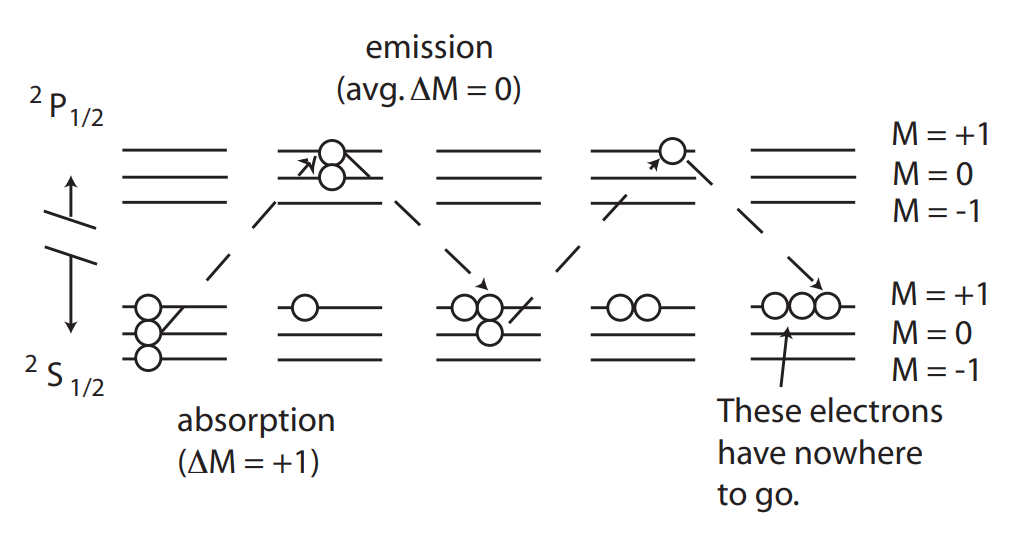
\includegraphics[scale=0.4]{figures/optic.png}
    \caption{Es ist das schematische Verhalten von Elektronen beim Optischen Pumpen von Wasserstoff im $F=1$ Niveau dargestellt.
    Die Energieniveaus sind jeweils der Grundzustand $^2S_{\sfrac{1}{2}}$ und der erste angeregte Zustand $^2P_{\sfrac{1}{2}}$.\cite{pdf_anleitung}}
    \label{fig:optic}
\end{figure}

\subsection{RF-Feld und Absorption}
Nach einer gewissen Zeit nimmt die Absorption des Rubidium Gases so stark ab, dass sie sich nicht mehr verändert.
In diesem Fall wurden alle Valenzelektronen auf das höchstmögliche Energieniveau gepumpt, sodass sie nicht mehr zur Absorption beitragen, und \autoref{eq:zeeman} bei angelegtem Magnetfeld gilt.
Um den Kernspin und den Landé-Faktor zu ermitteln wird ein RF-Feld angelegt, mit der Energie $E_\text{RF}$.\\
Sobald diese Energie gleich groß ist zur Wechselwirkungsenergie der Zeeman-Aufspaltung $\Delta E_{\text{Z},F}$, können die Elektronen zurück in einen günstigeren Energiezustand relaxieren.
Das wird als Absorptionsanstieg beobachtet, da nun mehr Elektronen an der Wechselwirkung teilnehmen.\\
Durch Umstellung der Formel
\begin{equation}
    E_\text{RF} = g_F \mu_B M B
    \label{eq:zeeman_frequenz}
\end{equation}
kann der Landé-Faktor ausgerechnet werden und dadurch auch der Kernspin.

\subsection{Rabi-Oszillationen}
Die Rabi-Oszillationen sind nach dem amerikanischen Physiker Isidor Isaac Rabi benannt.
In einem quantenmechanischen Zwei-Niveau-System kann die Besetzung dieser Zustände oszillieren, wenn die äußere Anregungsfrequenz gerade die Resonanzfrequenz $\omega_{21} = (E_2 -E_1)/\hbar$ der Zustände ist.
Die Frequenz dieser Besetzungsoszillation nennt sich Rabi-Frequenz.